En la Figura~\ref{fig:model_loss} se muestra la el valor de la p\'erdida MSE en funci\'on de la \'epoca de entrenamiento. \\

El mejor modelo de obtiene despu\'es de 175 \'epocas, con un valor de p\'erdida para el conjunto de datos de entrenamiento de 11276.5, para el conjunto de datos de validaci\'on de 11446.9, y para el conjunto de datos de testeo de 12357.7.  \\

\begin{figure}[h]
\centering
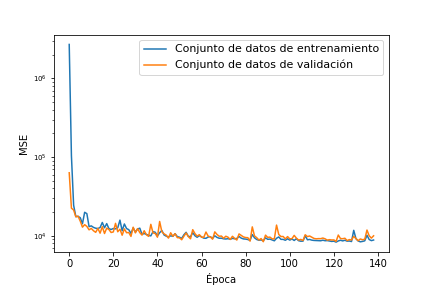
\includegraphics[width=0.8\textwidth]{figures/model_loss.png}
\caption{Valor del MSE en funci\'on de la \'epoca de entrenamiento para el conjunto de datos de entrenamiento (en azul) y para el conjunto de datos de validaci\'on (en naranja).}
\label{fig:model_loss}        
\end{figure}

En la Figura~\ref{fig:test_ptpred_genpt} se muestra la distribuci\'on bidimensional del momento transverso de predicho por la red en funci\'on del momento transverso de generaci\'on para los muones del conjunto de datos de testeo, directamente comparable con la Figura~\ref{fig:test_tuneppt_genpt}, donde se muestra para el mismo conjunto de datos el momento transverso dado por el algoritmo TuneP en funci\'on del momento transverso de generaci\'on. \\

\begin{figure}[h]
\centering
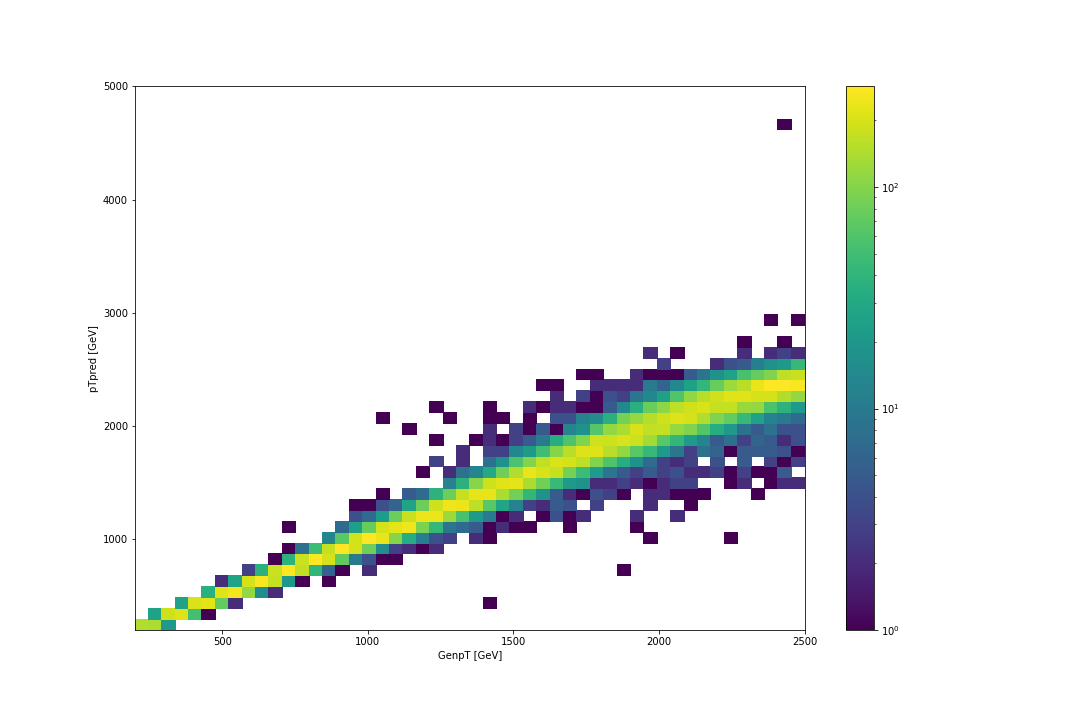
\includegraphics[width=1.0\textwidth]{figures/data_test_ptpred_genpt.png}
\caption{Distribuci\'on bidimensional del $p_{T}$ predicho por la red neuronal en funci\'on del $p_{T}$ de generaci\'on para los muones del conjunto de datos de testeo.}
\label{fig:test_ptpred_genpt}  
\end{figure}


\begin{figure}[h]
\centering
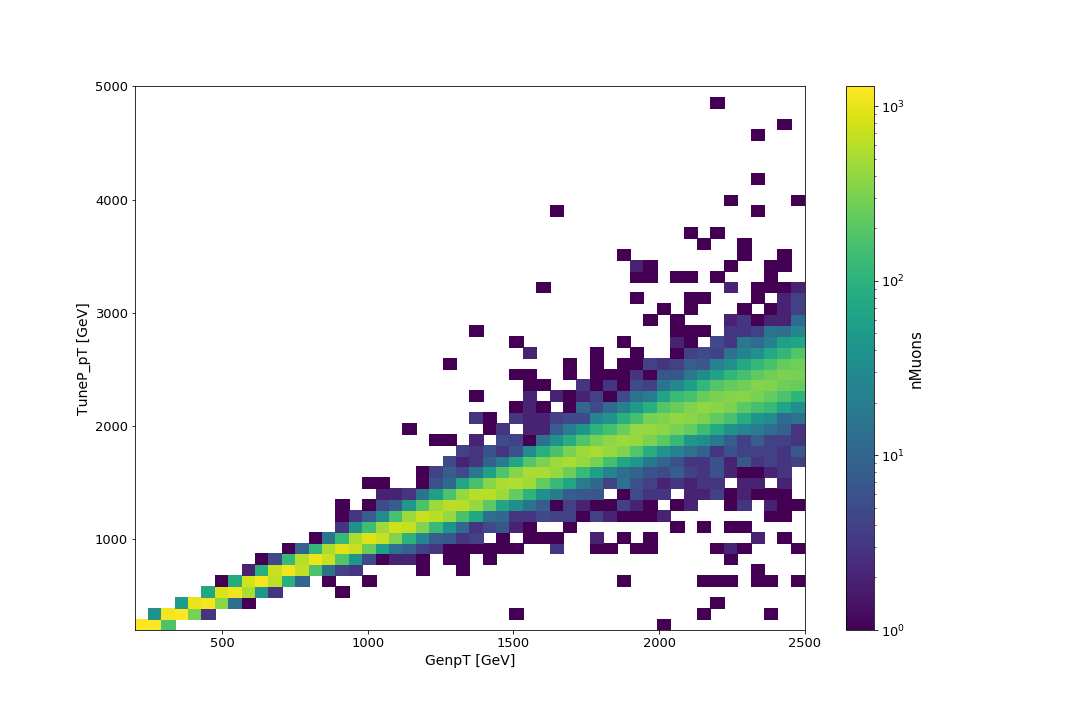
\includegraphics[width=1.0\textwidth]{figures/data_test_tuneppt_genpt.png}
\caption{Distribuci\'on bidimensional del $p_{T}$ dado por el algoritmo TuneP en funci\'on del $p_{T}$ de generaci\'on para los muones del conjunto de datos de testeo.}
\label{fig:test_tuneppt_genpt}  
\end{figure}

A la hora de cuantificar los resultados obtenidos ha de tenerse en cuenta que la red ha sido alimentada con muones generados con un valor m\'aximo para el $p_{T}$ de 2500 GeV, por tanto es natural pensar que el modelo va a tender a asignar un  $p_{T}$ igual o menor a este valor m\'aximo a los muones cuyo $p_{T}$ sea cercano a 2500 GeV. Por este motivo, y para tener resultados m\'as coherentes, la evaluaci\'on del m\'etodo se har\'a con muones con momento transverso generado en el rango 1800 $\leq p_{T} \leq$ 2300 GeV. \\


En la Figura~\ref{fig:R_predicted} se comparan la distribuciones de la resoluci\'on R, definida en \eqref{eq:R}, calculadas sobre el conjunto de datos de testeo con 1800 $\leq p_{T}^{GEN} \leq$ 2300 GeV, a partir del $p_{T}$ que da el algoritmo TuneP y a partir del $p_{T}$ que predice la red neuronal respectivamente. \\
Se obtiene un valor promedio para la resoluci\'on promedio en el conjunto de muones de testeo de R = 0.0575 $\pm$ 0.0012 usando el $p_{T}$ del algorimo TuneP, y de R = 0.04845 $\pm$ 0.0006 usando el $p_{T}$ predicho por el modelo de regresi\'on. Por lo tanto, se consigue una mejora en la asignaci\'on del momento transverso de aproximadamente un 20\% para estos muones altamente energ\'eticos.

\begin{figure}[h]
\centering
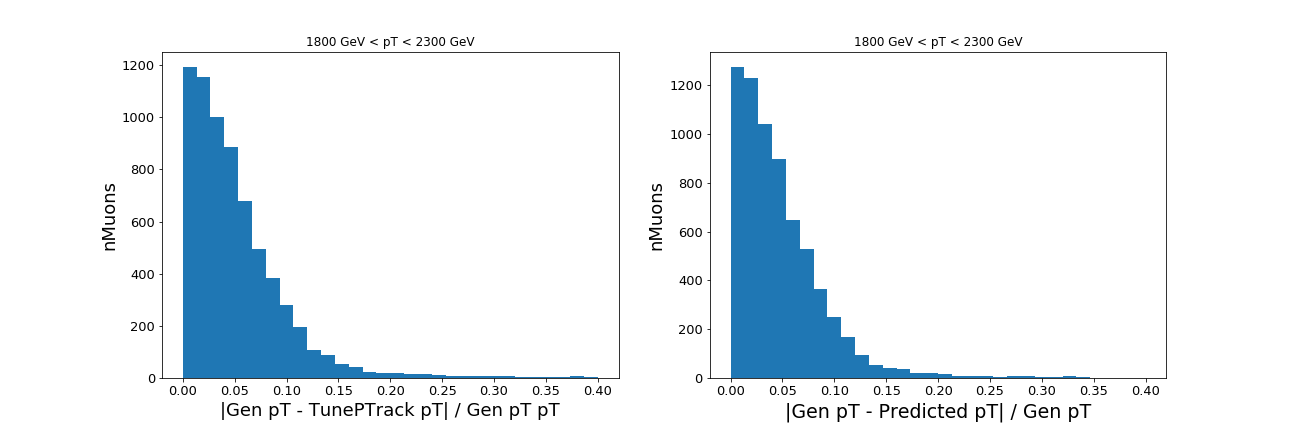
\includegraphics[width=1.2\textwidth]{figures/R_predicted_1800_2300.png}
\caption{Distribuci\'on de la resoluci\'on R dada por \eqref{eq:R} sobre el conjunto de muones de testeo con 1800 $\leq p_{T}^{GEN} \leq$ 2300 GeV. Izquierda: tomando el $p_{T}$ que da el algoritmo TuneP. Derecha: tomando el $p_{T}$ predicho por el modelo de regresi\'on al $p_{T}$.}
\label{fig:R_predicted}        
\end{figure}



\clearpage
